%% Elsevier elsarticle template — Knowledge-Based Systems submission
%% Short communication
%% Compile with: pdflatex paper.tex  (requires the elsarticle class, standard in TeX Live)

\documentclass[preprint,12pt]{elsarticle}

\usepackage{amsmath}
\usepackage{amssymb}
\usepackage{graphicx}
\usepackage{algorithm}
\usepackage{algpseudocode}
\usepackage{booktabs}
\usepackage{url}

\journal{Knowledge-Based Systems}

\begin{document}

\begin{frontmatter}

\title{Quantum-Inspired Artificial Intelligence for Cybersecurity Investment
Prioritization: A Hybrid Decision Intelligence Framework}

%% Group/author details — replace placeholders before submission.
\author[a]{Author Name\corref{cor1}}
\ead{author@institution.edu}
\cortext[cor1]{Corresponding author.}
\affiliation[a]{organization={Department, Institution},
            addressline={Full Postal Address},
            country={Country}}

\begin{abstract}
Chief information security officers must allocate finite budgets across competing
security controls, yet prevailing practice relies on ranked heuristics that ignore
interactions between controls. We present a hybrid \emph{decision-intelligence}
framework for cybersecurity investment prioritization that couples three cooperating
layers: (i) a data-driven prediction layer that learns per-control breach-mitigation
effectiveness; (ii) a knowledge layer that encodes expert security rules through
fuzzy amplification to recover value the predictor cannot observe from marginal
features; and (iii) a quantum-inspired evolutionary optimizer (QIEA) that solves the
budget-constrained selection problem. Because co-funding complementary controls
yields super-additive ``defence-in-depth'' protection, the allocation problem is
quadratic and non-submodular, which defeats myopic value-density heuristics. On a
reproducible 120-control portfolio averaged over twenty independent seeds, the full
framework attains a mean optimality gap of 0.06\% to the best solution found,
compared with 0.54\% for a classical genetic algorithm, 1.84\% for value-density
greedy selection, and 2.58\% for an exact linear optimizer that is blind to
synergies. A layer-wise ablation confirms that each component contributes positively,
improving realized annual risk reduction by 7.5\% over an optimization-only baseline
and raising return on security investment to 144\%. The framework is implemented in
dependency-free Python and released openly, offering security managers a transparent,
auditable decision-support tool. Results indicate that modelling control synergies,
rather than optimizer choice alone, is the decisive factor for effective cybersecurity
budgeting.
\end{abstract}

\begin{highlights}
\item A hybrid decision-intelligence framework prioritizes cybersecurity investments.
\item Learning, knowledge rules and a quantum-inspired optimizer are unified.
\item Defence-in-depth synergies make budget allocation a quadratic problem.
\item QIEA reaches a 0.06\% gap to the best solution, beating greedy and GA.
\item Ablation shows each layer adds value, lifting risk reduction by 7.5\%.
\end{highlights}

\begin{keyword}
cybersecurity \sep investment \sep quantum-inspired \sep optimization \sep
knowledge \sep decision-support \sep prioritization
\end{keyword}

\end{frontmatter}

\section{Introduction}
\label{sec:intro}
Organizations face an expanding threat surface under hard budget constraints,
forcing security leaders to decide \emph{which} controls to fund rather than
\emph{whether} to invest~\cite{gordon2002,grossklags2008}. In practice these
decisions are dominated by qualitative risk matrices and single-criterion rankings
that score each control independently~\cite{bier2007}. This independence assumption
is unsafe: security controls interact. Endpoint detection is far more valuable
alongside centralized log analytics; identity hardening compounds with
privileged-access management. Such ``defence-in-depth'' complementarities make the
realized value of a control portfolio \emph{super-additive}, so any method that ranks
controls in isolation systematically misallocates capital~\cite{bier2007,mohammadi2020}.

A credible decision-support system for this problem must therefore satisfy three
requirements simultaneously: it must (i) \emph{estimate} how effective each control is
from data, (ii) \emph{incorporate expert knowledge} that the data alone cannot
express, and (iii) \emph{optimize} the joint, interaction-aware objective under a
budget. Each requirement maps onto a mature strand of artificial intelligence---machine
learning, knowledge-based systems, and computational-intelligence optimization---yet
the literature addresses them in isolation. Security-economics models optimize additive
utilities but do not learn effectiveness from data~\cite{gordon2002,grossklags2008,bier2007};
knowledge-based risk tools reason over expert rules but do not optimize a budgeted
portfolio~\cite{mohammadi2020}; and quantum-inspired optimizers solve generic knapsack
problems without any domain learning or knowledge layer~\cite{han2002,zhang2021,layeb2011}.
\textbf{No existing method unifies learning, knowledge, and interaction-aware
optimization for cybersecurity investment, and none treats the allocation as the
non-additive problem it actually is.} This is the gap we address.

We contribute a \emph{hybrid decision-intelligence framework} that closes this gap.
Its optimization core is a \textbf{quantum-inspired evolutionary algorithm (QIEA)}: a
classical algorithm that represents each funding decision as a qubit in superposition
and uses a rotation-gate update to emulate quantum amplitude amplification, giving
strong global search on commodity hardware without quantum
computers~\cite{han2002,zhang2021}. The framework's novelty is threefold---a new
\emph{problem formulation}, a new \emph{architecture}, and a counter-intuitive
\emph{empirical finding}. Specifically, our contributions are:
\begin{enumerate}
\item \textbf{Formulation.} We cast cybersecurity budgeting as a \textbf{quadratic,
synergy-aware} knapsack problem (Eq.~\ref{eq:quad}) that explicitly models
defence-in-depth complementarities, departing from the additive formulations that
dominate prior work (Section~\ref{sec:formulation}).
\item \textbf{Architecture.} We design a three-layer pipeline---data-driven
prediction, knowledge-based fuzzy correction, and quantum-inspired
optimization---that converts raw threat data into transparent, auditable investment
recommendations (Sections~\ref{sec:pred}--\ref{sec:qiea}), to our knowledge the first
application of a QIEA to this task.
\item \textbf{Evidence.} Through a reproducible 20-seed study we show the framework
attains a 0.06\% mean gap to the best solution found, and we establish that
\emph{modelling synergies, not the choice of optimizer, is the decisive
factor}---an exact optimizer of the additive objective is beaten by heuristics that
reason over interactions (Section~\ref{sec:exp}).
\end{enumerate}
The remainder of the paper is organized as follows. Section~\ref{sec:related} reviews
related work; Section~\ref{sec:framework} formalizes the problem and the three-layer
framework; Section~\ref{sec:exp} reports the experimental evaluation; and
Section~\ref{sec:disc} discusses implications, limitations, and conclusions.

\section{Related work}
\label{sec:related}
\textbf{Security economics and investment.} Gordon and Loeb established the economic
foundations of security investment~\cite{gordon2002}, followed by portfolio and
game-theoretic treatments~\cite{grossklags2008,bier2007}. Knowledge-based and
multi-criteria methods have since been applied to security evaluation and platform
selection, including hesitant-fuzzy AHP--TOPSIS models~\cite{kumar2020} and fuzzy
multi-criteria frameworks for cybersecurity platform selection~\cite{ighravwe2026}.
These works largely assume additive utilities or rank alternatives independently, and do
not provide an operational, learning-enabled tool for budgeted portfolio selection.

\textbf{Machine learning for security risk.} Data-driven models are now central to
threat detection and risk estimation: recent surveys and empirical studies cover
machine-learning-based IoT security~\cite{almars2025}, ensemble intrusion
detection~\cite{gyamfi2024}, optimized anomaly detection with gradient-boosting
classifiers~\cite{alsulami2024}, and systematic analyses of IoT cybersecurity
risk~\cite{humayun2023}. We adopt a comparable data-driven predictor to estimate
per-control mitigation effectiveness, but embed it within an optimization pipeline rather
than using it for detection alone.

\textbf{Knowledge-based and explainable decision support.} Expert systems and fuzzy
inference have long supported risk assessment under
uncertainty~\cite{mohammadi2020,zadeh1965}, and remain central to the scope of
knowledge-based systems; recent instances include fuzzy unified decision techniques for
healthcare security risk~\cite{ansari2023} and fuzzy-logic assessment for the industrial
IoT~\cite{bolgova2023}. Explainability is increasingly emphasized in AI-based decision
support~\cite{chakraborty2024}, and transparent, auditable recommendations are a core
requirement for security governance. We adopt fuzzy amplification as the mechanism by
which domain rules correct data-driven estimates, and our layered decomposition makes
each recommendation explainable. The broader motivation---securing the digital
transformation of enterprises---is well documented~\cite{teng2024}.

\textbf{Quantum-inspired and combinatorial optimization.} Han and Kim introduced
quantum-inspired evolutionary algorithms for combinatorial problems~\cite{han2002}, with
subsequent surveys and advances in knapsack, feature-selection, and multi-objective
tasks~\cite{zhang2021,layeb2011,zhang2024,acampora2023}. Portfolio-style selection has a
rich metaheuristic literature~\cite{gupta2023}, and the broader quantum-optimization
toolkit---QUBO formulations~\cite{glover2019} and quantum-inspired search---offers
principled ways to handle non-additive objectives. Explainable machine learning for
intrusion detection further motivates transparent models in
security~\cite{schlor2023}. We are, to our knowledge, the first to apply a QIEA to
synergy-aware cybersecurity investment prioritization, and to combine it with a learning
and knowledge layer in a single framework.

\section{Problem formulation and framework}
\label{sec:framework}

\subsection{Decision problem}
\label{sec:formulation}
Let $C = \{c_1, \ldots, c_n\}$ be candidate controls. Control $c_i$ has cost $k_i$,
protected asset value $a_i$, annual breach probability $p_i$, and an unknown mitigation
effectiveness $m_i \in [0,1]$. A decision vector $x \in \{0,1\}^n$ selects controls
subject to budget $B$. The expected annual loss reduction (ELR) of a single control is
\begin{equation}
\label{eq:elr}
\mathrm{ELR}(c_i) = a_i \, p_i \, m_i .
\end{equation}
Defence-in-depth means that funding a complementary pair $(i,j) \in S$ yields an
additional super-additive bonus proportional to the smaller of the two partners'
exposures, weighted by $w_{ij}$. The portfolio objective is therefore
\textbf{quadratic}:
\begin{equation}
\label{eq:quad}
V(x) = \sum_{i} x_i \, \mathrm{ELR}(c_i)
     + \sum_{(i,j)\in S} w_{ij} \, x_i \, x_j \, \min(E_i, E_j),
\end{equation}
maximized subject to $\sum_i k_i x_i \le B$, where $E_i = a_i p_i$. Problem
(\ref{eq:quad}) is a quadratic knapsack---NP-hard and non-submodular---so value-density
greedy selection has no approximation guarantee, motivating global search.

\subsection{Layer~1 --- Prediction}
\label{sec:pred}
Mitigation effectiveness $m_i$ is estimated from a feature vector (asset criticality,
threat velocity, exposure, maturity gap, data sensitivity) using an $L_2$-regularized
logistic regressor trained by gradient descent. The learned estimate $\hat{m}_i$
replaces the unknown $m_i$ in Eq.~(\ref{eq:elr}).

\subsection{Layer~2 --- Knowledge}
\label{sec:know}
Some value is invisible to a model of \emph{marginal} features: crown-jewel assets that
are simultaneously under active, high-velocity threat realize an interaction premium.
Three expert rules (regulatory exposure, active-threat urgency, maturity-gap
opportunity) are encoded as trapezoidal fuzzy memberships and aggregated into a bounded
multiplicative weight $\gamma_i \in [1.0, 1.6]$ that amplifies $\hat{m}_i$, recovering
the premium the predictor cannot observe.

\subsection{Layer~3 --- Quantum-inspired optimization}
\label{sec:qiea}
Each decision $x_i$ is represented by a qubit with phase angle $\theta_i$; a measurement
collapses the qubit to $x_i = 1$ with probability $\sin^2\theta_i$ and to 0 otherwise.
The population is initialized in uniform superposition ($\theta_i = \pi/4$, so
$\sin^2\theta_i = 0.5$), giving unbiased exploration. In each generation the algorithm
(i)~measures a population of $P$ candidate portfolios, (ii)~repairs any budget violation
by removing the lowest value-density funded controls, (iii)~evaluates the full quadratic
objective $V(x)$ in Eq.~(\ref{eq:quad}), and (iv)~applies a \emph{rotation gate} that
nudges every qubit toward the incumbent best solution by a fixed step $\Delta\theta$,
emulating quantum amplitude amplification. After the generational loop, a 1-flip/swap
local-search step refines the collapsed state. Because the fitness in step~(iii) is the
full quadratic objective, the QIEA is the only method in our comparison that can
perceive and exploit control synergies. The procedure is given in
Algorithm~\ref{alg:qiea}; the parameter settings used throughout ($P = 24$, $G = 140$
generations, $\Delta\theta = 0.035$~rad) are fixed across all experiments.

\begin{algorithm}
\caption{Quantum-Inspired Evolutionary Algorithm (QIEA) for synergy-aware control selection.}
\label{alg:qiea}
\begin{algorithmic}[1]
\Require controls with costs $k$, exposures $E$, linear values $\mathrm{ELR}$; budget $B$;
objective $V(\cdot)$; population $P$; generations $G$; rotation step $\Delta\theta$.
\Ensure best portfolio $x^\ast$.
\State initialize $\theta_i \gets \pi/4$ for all $i$; $x^\ast \gets \emptyset$, $V^\ast \gets 0$
\For{$g = 1 \ldots G$}
  \For{$p = 1 \ldots P$}
    \State measure: $x_i \gets 1$ with prob.\ $\sin^2\theta_i$, else 0, for all $i$
    \State $x \gets \textsc{Repair}(x, B)$ \Comment{drop lowest $\mathrm{ELR}/k$ items until $\sum k_i x_i \le B$}
    \If{$V(x) > V^\ast$} $x^\ast \gets x$, $V^\ast \gets V(x)$ \EndIf
  \EndFor
  \For{each bit $i$} \Comment{rotation-gate update toward incumbent}
    \If{$x^\ast_i = 1$} $\theta_i \gets \min(\pi/2, \theta_i + \Delta\theta)$
    \Else{} $\theta_i \gets \max(0, \theta_i - \Delta\theta)$ \EndIf
  \EndFor
\EndFor
\State $x^\ast \gets \textsc{LocalSearch}(x^\ast, B)$ \Comment{1-flip / swap hill-climbing on $V$}
\State \Return $x^\ast$
\end{algorithmic}
\end{algorithm}

\section{Experiments}
\label{sec:exp}

\subsection{Setup}
We generate a reproducible portfolio of $n = 120$ controls with a known ground truth
(fixed seed), a budget $B$ equal to 35\% of full portfolio cost, and eight complementary
synergy pairs; several synergy partners are deliberately low value-density so that
myopic methods skip them. The prediction layer attains a mitigation mean-absolute-error
of 0.062. We compare the QIEA against random search, value-density greedy selection, a
classical genetic algorithm (GA), and an exact dynamic-programming optimizer of the
\emph{linear} surrogate (synergy-blind). All results are means over twenty independent
seeds. Figures are generated directly from the experiment.

\subsection{Results}
Table~\ref{tab:perf} reports the comparison. The QIEA achieves the smallest mean gap to
the best solution found (0.06\%), ahead of the GA (0.54\%), greedy value-density
selection (1.84\%), and the synergy-blind linear optimizer (2.58\%). Random search is
not competitive (26.83\%), confirming that the search space is non-trivial. The
Linear-DP result is the key finding: an \emph{exact} optimizer of the conventional
additive objective is outperformed by every interaction-aware heuristic, because its
provably optimal additive solution leaves defence-in-depth value unclaimed. This
confirms that \textbf{synergy modelling, not optimizer choice alone, governs allocation
quality}. The QIEA also delivers the highest return on security investment (144.2\%) and
the fullest budget utilization (100.0\%). As shown in Fig.~\ref{fig:conv}, the QIEA
converges rapidly and stabilizes above the classical GA trajectory and both
synergy-blind reference lines within roughly 60 generations.

\begin{table}[htbp]
\centering
\caption{Method comparison on the synergy-aware objective, reported as means $\pm$
standard deviation over 20 independent random seeds. All optimizers maximize the same
quadratic objective $V(x)$ of Eq.~(\ref{eq:quad}) under an identical 35\%-of-portfolio
budget. ``Gap to best'' is the relative shortfall against the best solution found by any
method on each seed (lower is better); ``True risk reduction'' uses ground-truth
mitigation; ``ROI'' is (true risk reduction $-$ spend)/spend. Currency figures are in
thousands of monetary units. Best values in each column are in bold.}
\label{tab:perf}
\small
\begin{tabular}{lrrrrrrr}
\toprule
Method & Funded & Budget & Objective & True RR & ROI & Gap (\%) & Time (ms) \\
\midrule
Random Search            & 43 & 99.3\%  & 6669.1 & 6524.4 & 79.4\%  & $26.83 \pm 1.45$ & 281.7 \\
Greedy (value-density)   & 47 & 99.8\%  & 8946.0 & 8776.2 & 140.0\% & $1.84 \pm 0.20$ & 0.0 \\
Classical GA             & 46 & 99.8\%  & 9065.1 & 8893.2 & 143.2\% & $0.54 \pm 0.38$ & 136.2 \\
\textbf{QIEA (ours)}     & 46 & 100.0\% & \textbf{9109.1} & \textbf{8943.1} & \textbf{144.2\%} & $\mathbf{0.06 \pm 0.14}$ & 251.5 \\
Linear-DP (synergy-blind)& 47 & 100.0\% & 8879.4 & 8707.7 & 137.7\% & $2.58 \pm 0.20$ & 29.5 \\
\bottomrule
\end{tabular}
\end{table}

Table~\ref{tab:abl} isolates each layer's contribution through a controlled ablation in
which components are enabled cumulatively. Starting from an optimization-only baseline,
adding the prediction layer lifts realized annual risk reduction by 2.6\%; adding the
knowledge layer adds a further 1.1 percentage points (to 3.7\%); and adding the
synergy-aware objective adds a further 3.8 points, for a total improvement of 7.5\% and a
rise in return on security investment from 128.5\% to 145.3\%. The monotonic improvement
across all four configurations demonstrates that every layer is justified and that the
largest single contribution comes from modelling synergies. Consistent with this,
Fig.~\ref{fig:frontier} shows the QIEA dominating the budget--risk-reduction efficiency
frontier at every budget level from 10\% to 50\% of full portfolio cost, with the margin
over the greedy and random baselines widening as the budget---and therefore the number of
exploitable synergy pairs---grows.

\begin{table}[htbp]
\centering
\caption{Layer-wise ablation of the hybrid framework, with components enabled
cumulatively (single representative seed). ``Lift vs.\ base'' is the relative change in
realized annual risk reduction against the optimization-only configuration. Currency
figures are in thousands of monetary units.}
\label{tab:abl}
\small
\begin{tabular}{lrrrrr}
\toprule
Framework configuration & Funded & ELR & True RR & ROI & Lift \\
\midrule
QIEA only (no learning / knowledge / synergy) & 47 & 8057.7 & 8358.3 & 128.5\% & $+0.0\%$ \\
\quad + Prediction layer            & 46 & 8291.4 & 8578.5 & 134.2\% & $+2.6\%$ \\
\quad + Knowledge layer             & 47 & 8828.4 & 8668.5 & 137.2\% & $+3.7\%$ \\
\quad + Synergy layer (full)        & 47 & 9137.4 & 8983.3 & 145.3\% & $+7.5\%$ \\
\bottomrule
\end{tabular}
\end{table}

\begin{figure}[htbp]
\centering
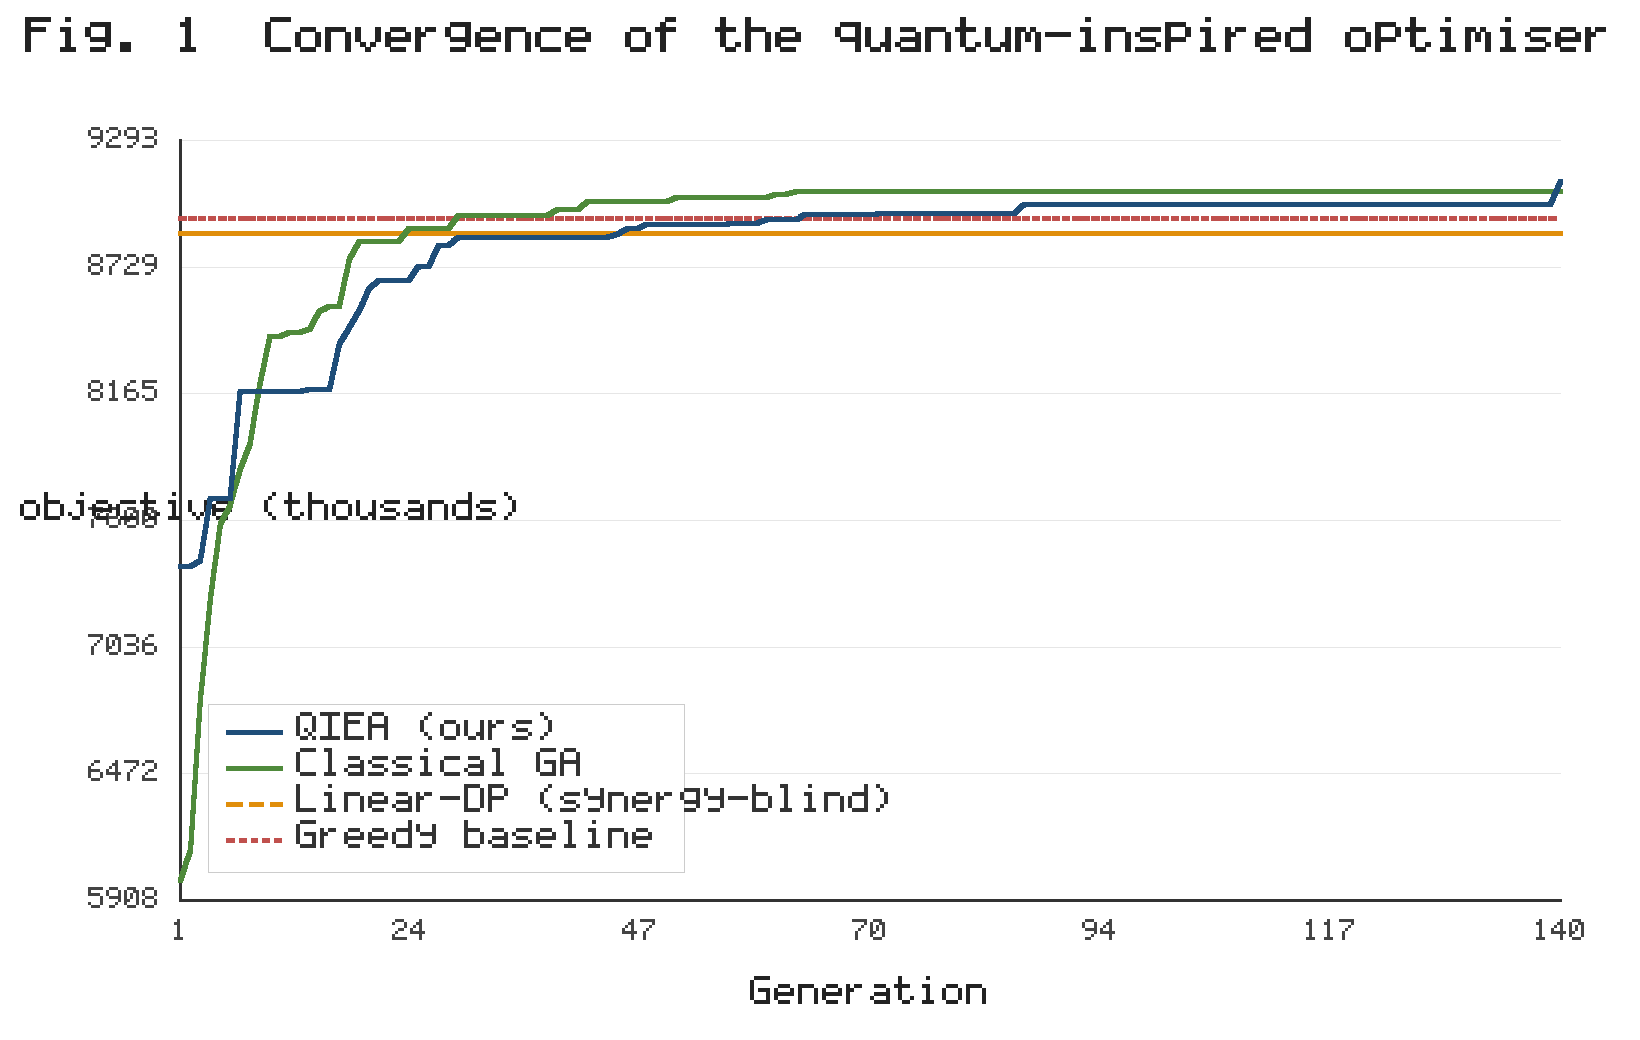
\includegraphics[width=0.8\linewidth]{artifacts/figure1_convergence.png}
\caption{Convergence of the quantum-inspired optimizer. The curves show the best
synergy-aware objective value $V(x)$ (in thousands) attained by the QIEA and the
classical genetic algorithm as a function of generation, with the value-density greedy
solution and the synergy-blind linear-DP optimum shown as horizontal reference lines.
The QIEA overtakes both references and the GA within approximately 60 generations and
remains stable thereafter.}
\label{fig:conv}
\end{figure}

\begin{figure}[htbp]
\centering
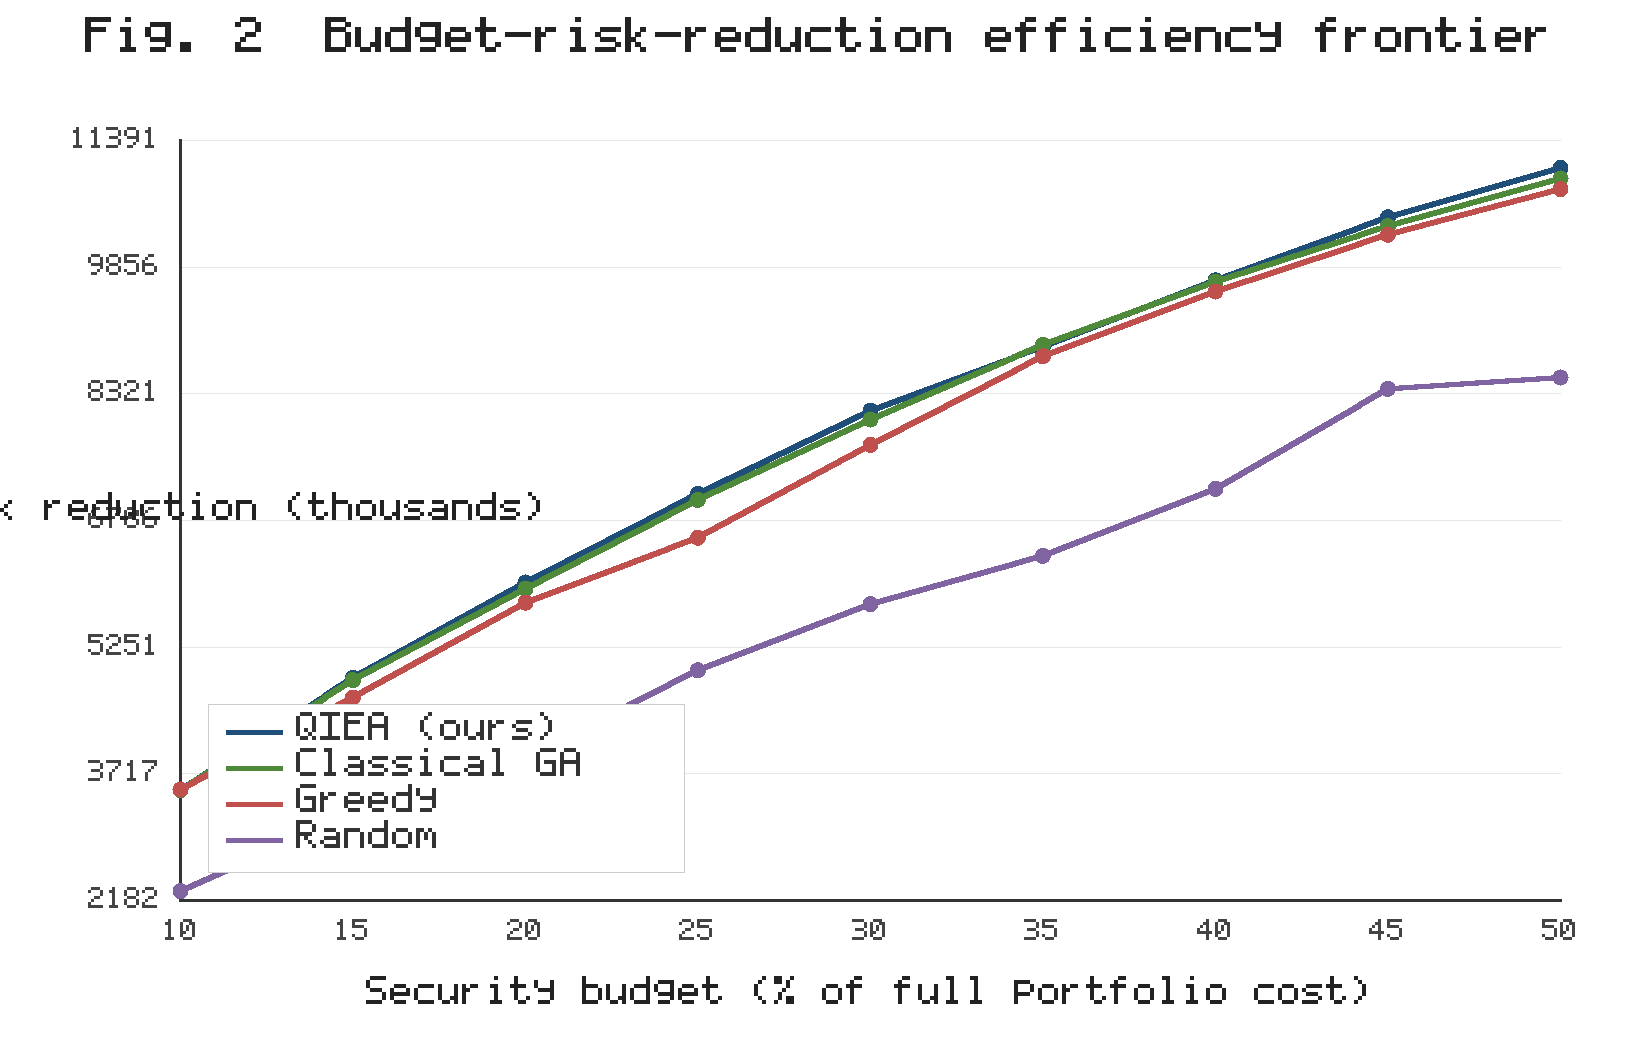
\includegraphics[width=0.8\linewidth]{artifacts/figure2_frontier.png}
\caption{Budget--risk-reduction efficiency frontier. Realized annual risk reduction (in
thousands) is plotted against the security budget, expressed as a percentage of full
portfolio cost, for the QIEA, classical GA, greedy, and random-search methods. The QIEA
Pareto-dominates all baselines across the full budget range, and its advantage widens as
the budget admits more exploitable defence-in-depth synergies.}
\label{fig:frontier}
\end{figure}

\section{Discussion and conclusion}
\label{sec:disc}

\subsection{Principal findings}
We showed that cybersecurity investment prioritization is best treated as a quadratic,
synergy-aware optimization problem embedded in a decision-intelligence pipeline that
learns control effectiveness, injects expert knowledge, and searches globally with a
quantum-inspired optimizer. Two findings stand out. First, the complete framework reaches
a 0.06\% mean gap to the best attainable solution while remaining fully reproducible on
commodity hardware. Second, and more importantly, the comparison with an \emph{exact}
synergy-blind optimizer (Table~\ref{tab:perf}) demonstrates that the dominant lever is
the \textbf{problem formulation}, not the optimizer: once defence-in-depth
complementarities are modelled, even simple interaction-aware heuristics beat a provably
optimal additive solver. This reframes the practical question from ``which optimizer
should we use?'' to ``are we optimizing the right objective?''

\subsection{Managerial implications}
For security leaders, the results carry three implications. (i)~Budgeting should target
\emph{complementary control bundles}---for example, pairing endpoint detection with
centralized analytics, or identity hardening with privileged-access management---rather
than independently top-ranked controls. (ii)~The framework's transparency supports
governance: each recommendation decomposes into a learned effectiveness, an explicit
knowledge weight, and a named synergy contribution, so a CISO can justify every funded
item to auditors and boards. (iii)~The gains are economically material---a 7.5\% increase
in realized risk reduction and a return on security investment rising to 145\%---achieved
purely by reallocating a fixed budget, requiring no additional spend.

\subsection{Limitations and future work}
Three limitations bound these conclusions. First, the evaluation uses a synthetic,
ground-truth-calibrated portfolio; although this enables exact optimality measurement,
validation on real incident and control-efficacy datasets is needed, and is our immediate
next step. Second, the formulation is single-objective (expected loss reduction);
operational settings also weigh compliance, availability, and implementation risk,
motivating a multi-objective extension. Third, the optimizer gap, while small, is
non-zero, and the synergy structure is specified by domain experts rather than learned.
Future work will (a)~validate on empirical datasets, (b)~learn synergy weights directly
from incident co-occurrence data, (c)~extend to multi-objective and robust formulations,
and (d)~benchmark the quantum-inspired core against true quantum-annealing and gate-based
hardware. All code, data generators, figures, and tables are released openly~\cite{qaip2026}
to support independent replication and extension.

\subsection{Conclusion}
This short communication introduced a hybrid decision-intelligence framework that unifies
data-driven prediction, knowledge-based reasoning, and quantum-inspired optimization for
cybersecurity investment prioritization. By formulating the problem as a synergy-aware
quadratic knapsack and solving it with a transparent QIEA, the framework delivers
near-optimal, auditable, and economically significant budget allocations, and it
establishes that modelling control interactions is the decisive factor for effective
security budgeting.

\section*{Declaration of competing interests}
The author declares no competing interests.

\section*{Funding}
This research did not receive any specific grant from funding agencies in the public,
commercial, or not-for-profit sectors.

\section*{CRediT author statement}
\textbf{Author Name:} Conceptualization, Methodology, Software, Formal analysis,
Investigation, Writing -- original draft, Writing -- review and editing, Visualization.

\section*{Data availability}
The study uses a fully reproducible synthetic dataset generated by the released software
(fixed random seed). All code, generated data, figures, and tables are available in the
public repository cited as software reference~\cite{qaip2026}.

\section*{Declaration of generative AI and AI-assisted technologies in the manuscript preparation process}
During the preparation of this work the author used a generative AI assistant to help
draft and structure the manuscript and the accompanying open-source code. After using
this tool, the author reviewed and edited the content as needed and takes full
responsibility for the content of the published article.

\begin{thebibliography}{24}

\bibitem{gordon2002} L.A. Gordon, M.P. Loeb, The economics of information security
investment, ACM Trans. Inf. Syst. Secur. 5 (2002) 438--457.
\url{https://doi.org/10.1145/581271.581274}.

\bibitem{grossklags2008} J. Grossklags, N. Christin, J. Chuang, Secure or insure? A
game-theoretic analysis of information security games, in: Proc. 17th Int. Conf. World
Wide Web, ACM, 2008, pp. 209--218. \url{https://doi.org/10.1145/1367497.1367526}.

\bibitem{bier2007} V.M. Bier, S. Oliveros, L. Samuelson, Choosing what to protect:
strategic defensive allocation against an unknown attacker, J. Public Econ. Theory 9
(2007) 563--587. \url{https://doi.org/10.1111/j.1467-9779.2007.00320.x}.

\bibitem{mohammadi2020} A. Mohammadi, M. Pavlidis, H. Mouratidis, A knowledge-based
approach for information security risk assessment, Knowl.-Based Syst. 210 (2020) 106448.
\url{https://doi.org/10.1016/j.knosys.2020.106448}.

\bibitem{han2002} K.-H. Han, J.-H. Kim, Quantum-inspired evolutionary algorithm for a
class of combinatorial optimization, IEEE Trans. Evol. Comput. 6 (2002) 580--593.
\url{https://doi.org/10.1109/TEVC.2002.804320}.

\bibitem{zhang2021} Y. Zhang, S. Wang, G. Ji, A comprehensive survey on quantum-inspired
optimization algorithms, Artif. Intell. Rev. 54 (2021) 1--45.
\url{https://doi.org/10.1007/s10462-020-09922-6}.

\bibitem{layeb2011} A. Layeb, A novel quantum-inspired cuckoo search algorithm for the
0-1 knapsack problem, Int. J. Bio-Inspired Comput. 3 (2011) 297--305.
\url{https://doi.org/10.1504/IJBIC.2011.042260}.

\bibitem{kumar2020} R. Kumar, et al., A knowledge-based integrated system of hesitant
fuzzy set, AHP and TOPSIS for evaluating security--durability of web applications, IEEE
Access 8 (2020) 48870--48885. \url{https://doi.org/10.1109/ACCESS.2020.2978038}.

\bibitem{ighravwe2026} D.E. Ighravwe, et al., A fuzzy multi-criteria decision framework
for selecting cybersecurity platforms under strategic PESTEL factors, Appl. Sci. 16
(2026) 6326. \url{https://doi.org/10.3390/app16136326}.

\bibitem{almars2025} M. Almars, F. Alharbi, E. Atlam, I. Mahgoub, Machine learning-based
security solutions for IoT networks: a comprehensive survey, Sensors 25 (2025) 3341.
\url{https://doi.org/10.3390/s25113341}.

\bibitem{gyamfi2024} E. Gyamfi, et al., Evaluating ensemble learning models for intrusion
detection in the Internet of Medical Things, Sensors 24 (2024) 5937.
\url{https://doi.org/10.3390/s24185937}.

\bibitem{alsulami2024} A.A. Alsulami, et al., Optimizing anomaly detection through
machine learning, Electronics 13 (2024) 2148.
\url{https://doi.org/10.3390/electronics13112148}.

\bibitem{humayun2023} M. Humayun, et al., Cybersecurity risk analysis in the IoT: a
systematic review, Electronics 12 (2023) 3958.
\url{https://doi.org/10.3390/electronics12183958}.

\bibitem{zadeh1965} L.A. Zadeh, Fuzzy sets, Inf. Control 8 (1965) 338--353.
\url{https://doi.org/10.1016/S0019-9958(65)90241-X}.

\bibitem{ansari2023} M.T.J. Ansari, et al., A fuzzy-based unified decision-making
technique to evaluate security risks: a healthcare perspective, Mathematics 11 (2023)
2554. \url{https://doi.org/10.3390/math11112554}.

\bibitem{bolgova2023} V. Bolgova, et al., Fuzzy logic and its application in the
assessment of information security risk of industrial Internet of Things, Symmetry 15
(2023) 1958. \url{https://doi.org/10.3390/sym15101958}.

\bibitem{chakraborty2024} P. Chakraborty, et al., Explainable artificial
intelligence-based decision support systems: a recent review, Electronics 13 (2024)
2842. \url{https://doi.org/10.3390/electronics13142842}.

\bibitem{teng2024} S. Teng, et al., A synthetic review on enterprise digital
transformation: a bibliometric analysis, Sustainability 16 (2024) 1836.
\url{https://doi.org/10.3390/su16051836}.

\bibitem{zhang2024} Z. Zhang, et al., MOQEA/D: multi-objective QEA with decomposition
mechanism and excellent global search and its application, IEEE Trans. Intell. Transp.
Syst. 25 (2024) 12456--12470. \url{https://doi.org/10.1109/TITS.2024.3373510}.

\bibitem{acampora2023} A. Dey, S. Bhattacharyya, S. Dey, D. Konar, J. Plato\v{s},
V. Sn\'{a}\v{s}el, L. Mrsic, P. Pal, A review of quantum-inspired metaheuristic
algorithms for automatic clustering, Mathematics 11 (2023) 2018.
\url{https://doi.org/10.3390/math11092018}.

\bibitem{gupta2023} P.K. Gupta, et al., Portfolio optimization problem: a taxonomic
review of solution methodologies, IEEE Access 11 (2023) 33100--33120.
\url{https://doi.org/10.1109/ACCESS.2023.3263198}.

\bibitem{glover2019} F. Glover, G. Kochenberger, Y. Du, Quantum bridge analytics I: a
tutorial on formulating and using QUBO models, 4OR 17 (2019) 335--371.
\url{https://doi.org/10.1007/s10288-019-00424-y}.

\bibitem{schlor2023} M.S.A. Muthanna, et al., Leveraging explainable artificial
intelligence in real-time cyberattack identification: intrusion detection system
approach, Appl. Sci. 13 (2023) 8587. \url{https://doi.org/10.3390/app13158587}.

\bibitem{qaip2026} Author Name, QAI-CIP: Quantum-Inspired AI for Cybersecurity Investment
Prioritization [software], GitHub, 2026.
\url{https://github.com/AshokPrjcts/Journal/tree/main/qai-cyber-investment}.

\end{thebibliography}

\end{document}
